\chapter{Применение векторно"--~алгебраического метода для изучения пространственно-временной изменчивости дрейфа морского льда и валидации модельных расчетов в Северном Ледовитом океане} \label{chapt3}


В главе рассматриваются теоретические основы векторно"~алгебраического метода, демонстрируется его применение для анализа временных рядов векторов дрейфа льда полученных на основе анализа спутниковых данных. Векторно"--~алгебраический подход позволяет существенно сжимать исходную информацию и наиболее адекватно описывать временные векторные ряды натурных и модельных данных ограниченным набором статистических характеристик в инвариантной форме.

\section{Использованные данные} \label{sect3_1}

Описание методики векторно"~алгебраического вероятностного анализа в данной статье проиллюстрировано примерами обработки временных рядов скоростей дрейфа льда в Северном Ледовитом океане, полученных по спутниковым изображениям для точек с фиксированными координатами и осредненными за сутки, и за календарный месяц. Тестовые расчеты были выполнены для рядов среднесуточных значений дрейфа в трех точках с 4.10.2007 по 30.04.2008 (продолжительность рядов около полугода) и для шести точек со среднемесячными данными с января 1979 г. по декабрь 2006 г. (продолжительность рядов 28 лет), см. табл.~\ref{tbl:tbl_points_drift_vam}, рис.~\ref{img:ivanov_01}а.
% TODO: Добавить ссылки на картинку

\begin{table} [htbp]%
	\centering
	\caption{Координаты точек, для которых выполнялись тестовые расчеты}%
	\label{tbl:tbl_points_drift_vam}% label всегда желательно идти после caption
	\renewcommand{\arraystretch}{1.5}%% Увеличение расстояния между рядами, для улучшения восприятия.
	\setlength{\tymax}{1.9cm}
	\begin{SingleSpace}
		\begin{tabular}{@{}@{\extracolsep{0pt}}lllllll@{}} %Вертикальные полосы не используются принципиально, как и лишние горизонтальные (допускается по ГОСТ 2.105 пункт 4.4.5) % @{} позволяет прижиматься к краям
			\toprule     %%% верхняя линейка
			№ точки & Широта & Долгота & № точки & Широта & Долгота &\\
         			&$^\circ~N$ &$^\circ~E,W$ &  &$^\circ~N$ &$^\circ~E,W$ &\\
       				& Среднесуточные& данные  & Среднемесячные & данные &\\
			\midrule %%% тонкий разделитель. Отделяет названия столбцов. Обязателен по ГОСТ 2.105 пункт 4.4.5 
			1	&82,18	&117,63~Е &4 &78,64	&125,94~E &\\
			2	&83,57	&124,39~W &5 &81,06	&137,04~W &\\
			3	&82,64	&70,63~E  &6 &85,04	&180,00~E &\\
				&   	&         &7 &84,62	&56,98~E &\\
				&   	&         &8 &81,20	&1,47~W &\\
				&   	&         &9 &78,99	&15,46 W &\\		
			
     	  \midrule%%% тонкий разделитель
			\multicolumn{7}{@{}p{\textwidth}}{%
				\vspace*{-4ex}% этим подтягиваем повыше
				\hspace*{2.5em}% абзацный отступ - требование ГОСТ 2.105
				Примечание "---  Положение этих точек приведено ниже на картах рис.~\ref{img:ivanov_01}a и ...
			}
			\\
			
			\bottomrule %%% нижняя линейка
			
		\end{tabular}%
	\end{SingleSpace}
\end{table}

\section{Методика анализа и обсуждение примеров ее применения} \label{sect3_2}
Анализ данных выполняется в терминах моделей векторной случайной величины, векторного стационарного случайного процесса, тренда математического ожидания и системы двух связных векторных случайных величин.

Поскольку ветер, морские течения, дрейф льда представляют собой направленный перенос массы, их скорости являются физическими векторами, то за модель скорости здесь принят евклидов вектор $\vec{V}$ с декартовыми проекциями  $V_x$, $V_x$, "--- математический объект, характеризуемый модулем $V$ и направлением $\phi$, для которого определены сложение по правилу параллелограмма, правила преобразования составляющих вектора при переходе к новой системе координат и три вида умножения векторов "--- скалярное, векторное (косое) и тензорное~\cite{Kochin2013}. Основанный на этих положениях  векторно-алгебраический метод~\cite{Belyshev1983} позволяет рассматривать данные в терминах моделей векторной случайной величины, векторного случайного процесса, системы связных векторных случайных величин и векторного пространственно"~временного случайного поля. Поскольку характеристики векторов многомерны (векторы и тензоры), обсуждаются не только вычислительные процедуры, но и способы цифрового и графического представления результатов.

\subsection{Модель векторной случайной величины}
В модели векторной случайной величины (СВ) значения скорости дрейфа $\vec{V}$ в фиксированных точках представлены статистическими оценками распределения вероятностей и его моментов~\cite{Belyshev1983,Klevancov1996}. Исчерпывающей вероятностной характеристикой стохастического вектора $\vec{V}$ как СВ является двумерное по модулю и направлению распределение, и маргинальные распределения вероятностей. Соответствующие повторяемости $P(V,\phi)$ определены как вероятности попадания значений $\vec{V}$ в заданную градацию $f(\bullet)$ 

\begin{equation}
\label{eq:equation3_1}
 \begin{alignedat}{2}
  P(V,\phi) = f\{V_1\le V<V_2, \phi_1\le\phi_2\},\\
  P(V) = f\{V_1\le V<V_2\},\\
  P(\phi) = f\{\phi_1\le \phi<\phi_2\} 
 \end{alignedat}
\end{equation}

Эти характеристики традиционно представляют таблицей двумерной и маргинальных повторяемостей по румбам и градациям модуля (повторяемость штиля выделяют в самостоятельную градацию). Такое представление, будучи весьма полезным в силу большой информативности, может быть использовано из"~за большой многомерности только для очень ограниченного набора точек пространства в характерные сезоны. Так, при выделении 16 градаций по направлению и 10 градаций по модулю "---  скорости дрейфа для каждой точки и для каждого сезона получаем таблицу двумерной повторяемости $f(V,\phi)$ из 160 (16$\times$10) ячеек и 2 таблицы маргинальных повторяемостей $f(\phi)$, $f(V)$ из 16 и 10 ячеек соответственно. В графической форме эти характеристики представляют полем $f(V,\phi)$ и графиками $f(\phi)$, $f(V)$ "--- рис.~\ref{img:ivanov_01}а.

\begin{figure}[ht] 
	\centering
	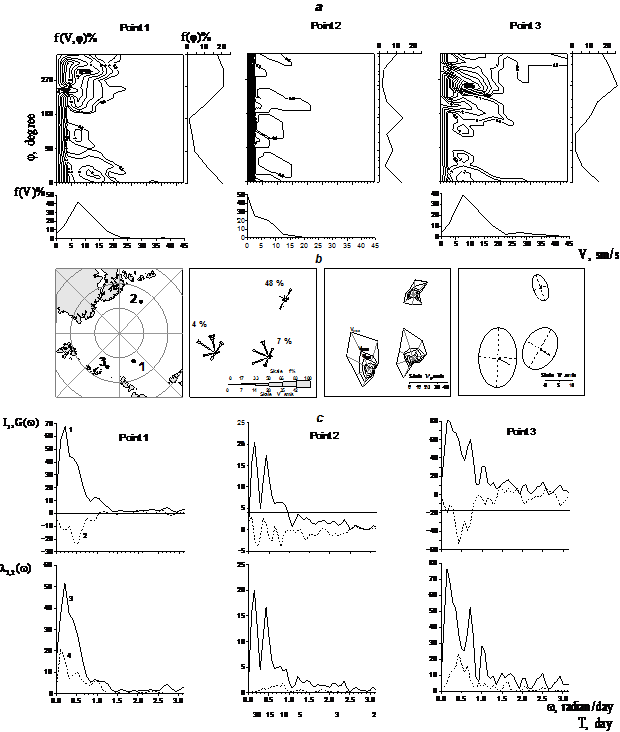
\includegraphics [scale=0.085] {ivanov_01}
	\caption{Вероятностные характеристики изменчивости среднесуточной скорости дрейфа в  точках № 1, 2 и 3. a "--- графики двумерной и маргинальных повторяемостей; b (слева направо): карта расположения точек, розы повторяемости (цифрами обозначена повторяемость отсутствия дрейфа), квантильные розы, векторы средней скорости и эллипсы СКО; c "--- инварианты спектрального тензора, 1 и 2 "--- инварианты $I_1$ и $G$, 3 и 4 "--- инварианты $\lambda_1$ и $\lambda_2$, внизу подписаны периоды $T$, соответствующие круговой частоте $\omega$.
	}
	\label{img:ivanov_01}
\end{figure}

Рис.~\ref{img:ivanov_01}а демонстрирует принципиальное различие распределений в точках 1, 3 сравнительно с точкой 2. В точке 2 наиболее часто отмечается отсутствие дрейфа и медленный дрейф "--- повторяемость штиля составляет около 50$\%$, а обеспеченность (накопленная повторяемость) скоростей до 5 см/с и до 10 см/с "--- 75$\%$ и 95$\%$ соответственно; распределение по румбам не имеет чётко выраженных мод. В точках 1, 3 распределение характеризуется хорошо выраженными модами. Максимальную повторяемость имеет дрейф с модулем скорости 5"--~15 см/с "--- суммарно около 70$\%$, направленный на W"~NW"~N. Основная мода распределения хорошо выделяется в поле двумерной повторяемости; некоторое различие точек 1 и 3 проявляется в том, что в точке 3 распределение является более сосредоточенным в окрестностях основной моды и более широким в области больших скоростей. Распределение по румбам среднего и максимального модуля скорости также имеет чёткие максимумы, которые согласованы с максимумом повторяемости, но полностью не совпадают с ними. Полученные характеристики дрейфа льда в каждой из точек хорошо согласуются с существующими представлениями о структуре и характере дрейфа в этих районах.

Для картирования лучше использовать розы повторяемости, но в этом случае количество румбов (градаций направления) должно быть 4 или 8, количество градаций модуля также не должно быть слишком большим. Карта роз повторяемости для точек 1"--~3 приведена на рис.~\ref{img:ivanov_01}b (второй слева фрагмент), в нижнем правом углу приведена масштабная линейка с обозначением градаций модуля скорости (ниже линейки) и масштаба повторяемости (выше линейки). Розы построены без учёта повторяемости штиля, так что резкое уменьшение размера розы соответствует частым штилевым ситуациям (точка 2). Повторяемость штиля для каждой точки дана на рисунке цифрами.

Так как при картировании полей, заданных на большом количестве точек, используется мелкий масштаб, розы повторяемости наиболее наглядно показывают   преобладающие направления скорости и румбы, для которых характерен наиболее быстрый дрейф, а анализ самих высоких скоростей затруднён. Для более детального описания скоростей дрейфа воспользуемся квантильной розой "--- третий слева фрагмент на рис.~\ref{img:ivanov_01}b. Для каждого румба $\phi$ составляется отдельная выборка. Квантилем модуля скорости $V_p$ порядка $р$ является корень уравнения $F(V)=p$, где $F(V)$ "--- обеспеченность, т.~е. $V_p$ "--- величина, обратная накопленной вероятности. Для построения квантильной розы (рис.~\ref{img:ivanov_01}b правее розы повторяемости) квантили $V_{min}$, $V_{0,25}$, $V_{0,50}$, $V_{0,75}$, $V_{max}$  отложены на соответствующих румбам $\phi$ лучах и соединены огибающими линиями. Две внешние огибающие $V_{0,75}$, $V_{max}$ показывают область 25$\%$ самых больших скоростей. Сравнение карт квантильных роз с розами повторяемости на рис.~\ref{img:ivanov_01}b, показывает, что в точках 1 и 3 наиболее высокие скорости имеет дрейф,  направленный на $N$ и на $NW$ соответственно, эти направления согласованы с румбами максимальной повторяемости, но полностью с ними не совпадают. Таким образом, розы повторяемости и квантильные розы являются не взаимно заменяющими, а наоборот взаимно дополнительными характеристиками.

Для сжатия информации мы использовали концепцию векторно"~алгебраического подхода~\cite{Belyshev1983}. Для описания распределения вероятностей при этом обычно используются моменты распределения, ограничиваясь чаще всего первым начальным моментом "--- математическим ожиданием и вторым центральным моментом "--- дисперсией. Математическое ожидание определено как вектор $\vec{m}_{\vec{V}}$, проекции которого равны математическим ожиданиям $(m_{V_x},m_{V_y})$ проекций вектора $\vec{V}$

\begin{equation}
\label{eq:equation3_2}
\vec{m}_{\vec{V}}=M\{V_X\vec{e}_X+V_Y\vec{e}_Y\},
\end{equation}
где $\vec{e_X}$ и $\vec{e_Y}$ "--- орты осей $OX$, $OY$. Это определение совпадает с определением средней скорости в покомпонентном методе, в котором моделью скорости является матрица"~строка $(m_{V_X},m_{V_Y})$ или соответствующая матрица"~столбец.

Определение дисперсии введено на основе более общего определения корреляционной функции, которая совместно с распределением \labelcref{eq:equation3_1} даёт исчерпывающую характеристику $\vec{V}(t)$ как векторного случайного процесса. Корреляционная функция в стационарном приближении $K_{\vec{V}(\tau)}$ определена как математическое ожидание $M$ тензорного произведения $\otimes$ центрированных векторов, сдвинутых на промежуток времени  

\begin{equation}
\label{eq:equation3_3}
K_{\vec{V}}(\tau)=M\{\vec{V}^0(t) \otimes \vec{V}^0(t+\tau)\},
\end{equation}

Функция $K_{\vec{V}}(\tau)$ характеризует взаимосвязь направленных изменений скорости в моменты времени, сдвинутые на интервал $\tau$ и даёт количественную меру их интенсивности и ориентацию в заданной системе координат.

Для плоских векторов $\vec{V}$ при фиксированном временном сдвиге $K_{\vec{V}}(\tau)$ есть тензор второго ранга с матрицей, элементы которой представлены ковариациями соответствующих проекций. Этот тензор может быть разложен единственным образом на сумму симметричного и кососимметричного тензоров

% подправить формулу (неровно подписи в скобках)
\begin{equation}
\label{eq:equation3_4}
{K_{\vec{V}(\tau)} = {{K_{V_{x}V_{x}}(\tau)\quad K_{V_{x}V_{y}}(\tau)}\choose {K_{V_{y}V_{x}}(\tau)\quad  K_{V_{y}V_{y}}(\tau)}}= C(\tau) + G(\tau) ={{{\lambda_{1}(\tau)\quad 0}} \choose 0\quad {\lambda_{2}(\tau)}}} + {0.5G(\tau){{0}\quad {1}\choose {-1}\quad {0}}}
\end{equation}

Если в покомпонентном методе ковариацией является матрица, каждый элемент которой имеет самостоятельное значение, то тензор "--- единый объект, инвариантный относительно преобразования исходной системы координат, а матрица в  \labelcref{eq:equation3_4} "--- только форма его записи. Компоненты тензора $K_{\vec{V}}(\tau)$  в общем случае зависят от выбора системы координат, но существуют инварианты "--- скалярные функционалы компонентов, не зависящие от изменения системы координат. Инвариантами $\lambda_{1,2}(\tau)$ симметричной части $C$ являются собственные числа  

\begin{equation}
\label{eq:equation3_5}
\lambda_{1,2}=0.5 \{ I_1 \pm \sqrt{(K_{V_x}-K_{V_y})^2 + 2K_{V_x V_y}^2}\},
\end{equation}   

а сам тензор $C$ приводится к симметричному виду разворотом исходной системы координат на угол

\begin{equation}
\label{eq:equation3_6}
\alpha=0.5\arctg{\frac{2K_{{V_{x}V_{y}}}} {K_{V_{x}}-K_{V_{y}}}}\pm180^{\circ} 
\end{equation}   

Инвариант кососимметричного тензора

\begin{equation}
\label{eq:equation3_7}
G=K_{{V_{x}V_{y}}}-K_{{V_{y}V_{x}}}
\end{equation} 

назван индикатором вращения, а сумма $\lambda_{1,2}$ названа линейным инвариантом $I_1$ 

\begin{equation}
\label{eq:equation3_8}
I_1=\lambda_{1}+\lambda_{2}
\end{equation}

Поскольку в формулы (3.4"--~3.8) входят все элементы матрицы $K_{\vec{V}}(\tau)$, они подчеркивают единство $K_{\vec{V}}(\tau)$ как абстрактного математического объекта в отличие от корреляционной матрицы, каждый элемент которой имеет самостоятельное значение. Сами же инварианты характеризуют различные свойства изменчивости.
Дисперсия есть значение ковариационной функции при нулевом временном сдвиге $D_{\vec{V}}\equiv{K_{\vec{V}}(0)}$. Поскольку взаимные ковариации проекций в этом случае равны ${K_{{V_{x}V_{y}}}(0)={K_{{V_{y}V_{x}}}(0)$, тензор дисперсии $D_{\vec{V}}$ является симметричным
		
\begin{equation}
\label{eq:equation3_9}
D_{\vec{V}} = {{{D_{V_{x}}\quad K_{V_{x}V_{y}}}\choose {K_{V_{y}V_{x}}\quad D_{V_{y}}}} = {{\lambda_1}\quad 0 \choose 0 \quad {\lambda_2}}}
\end{equation}	
		
и его линейный инвариант $I_1$ определяет общую интенсивность изменчивости $\vec{V}$ за счёт изменений как модуля, так и направления. 
Тензор среднеквадратического отклонения (СКО) $\sigma_{\vec{V}}$ определён как 
		
\begin{equation}
\label{eq:equation3_10}
\sigma_{\vec{V}} = \sqrt{D_{\vec{V}}} = {{\lambda^{(\sigma)}_1 \quad 0}\choose {\lambda^{(\sigma)}_2}}
\end{equation}
		
Его собственные числа являются квадратными корнями соответствующих собственных чисел тензора $D_{\vec{V}}-{{\lambda^{(\sigma)}}_{1,2}}}={\sqrt{{\lambda^{(D)}}_{1,2}}}$, следовательно, линейные инварианты тензоров $\sigma_{\vec{V}}$ и $D_{\vec{V}}$ не совпадают ${I^{(\sigma)}_1}={{\lambda^{(\sigma)}_1}+{\lambda^{(\sigma)}_2}\neq{\sqrt{I^{(D)}_1}}}$. В дальнейшем для тензора $\sigma_{\vec{V}}$ будем использовать обозначения $\lambda_{1,2}$ без верхнего индекса, а для характеристики общей изменчивости будем использовать $\sqrt{I^{(D)}_1$, обозначая его для общности как $I^{0.5}_1$. Выбор между $I^{(\sigma)}_1$ и $\sqrt{I^{(D)}_1}$ в пользу последнего связан, в частности, с возможностью ввести векторный коэффициент вариации (в знаменателе модуль вектора математического ожидания)
		
\begin{equation}
\label{eq:equation3_11}
v=\frac{\sqrt{I^{(D)}_1}}{m_{\vec{V}}}
\end{equation} 

Если $v>1$ "--- движение неустойчивое и наоборот. Используем также число
		
\begin{equation}
\label{eq:equation3_12}
\gamma={D_{V}}/{I^{(D)}_1}
\end{equation} 
		
Поскольку $I_1$ "--- общая дисперсия, а $D_V$ "--- дисперсия модуля скорости, то дополнение $\gamma$ до 1 (число 1-$\gamma$) определяет вклад изменчивости направления $\vec{V}$ в общую дисперсию.
Геометрическим образом $\sigma_{\vec{V}}$ является эллипс с полуосями $\lambda_{1,2}$ \labelcref{eq:equation3_5}, ориентированный в направлении максимальной изменчивости $\alpha$ \labelcref{eq:equation3_6}. Это Это также подчёркивает достоинство векторно-алгебраического метода сравнительно с покомпонентным методом, в котором направление максимальной изменчивости можно определить только в рамках априорной гипотезы о виде распределения проекций (например, двумерное нормальное распределение). Графически (как для отдельных точек, так и на картах) $\sigma_{\vec{V}}$ представляют овалом и/или осями эллипса, полезно совмещать его с вектором средней скорости $\vec{m}_{\vec{V}}$. Форму эллипса характеризует инвариант
	
\begin{equation}
\label{eq:equation3_13}
\chi=\lambda_{2}/\lambda_{1}
\end{equation} "--- показатель вытянутости. При $\chi=1$ эллипс превращается в окружность, что означает одинаковую по всем направлениям интенсивность изменчивости, а при $\chi=0$ эллипс вырождается в отрезок прямой, что означает реверсивные изменения $\vec{V}$ или изменения только модуля при постоянном направлении.
Такое представление, являющееся воплощением векторно-алгебраического подхода, обеспечивает очень существенное сжатие информации. Вместо громоздких таблиц повторяемости характеристика изменчивости временного ряда векторного процесса может быть представлена всего лишь 11 числами (табл.2) "--- модулем и направлением средней и максимальной скорости, инварианта $I^{0.5}_1$ тензора $D_{\vec{V}}$, параметрами эллипса СКО $\lambda_1$, $\lambda_2$, $\chi$, $\alpha$, коэффициентом изменчивости $v$ и относительной дисперсией $1-\gamma$, обусловленной изменениями направления дрейфа. Поскольку для эллипсов СКО противоположные направления $\alpha\pm180^{\circ}$ равноправны, 3 для эллипса $\sigma_{\vec{V}}$ выбрано значение $\alpha$, ближайшее к направлению среднего переноса. Для максимального сжатия информации и картирования можно ограничиться всего лишь 5 параметрами вектора: $\vec{m}_{\vec{V}}$ (2 числа) и эллипса СКО (3 числа). Векторы $\vec{m}_{\vec{V}}$ и эллипсы $\sigma_{\vec{V}}$ графически совмещены на правой карте рис.~\ref{img:ivanov_01}b.
 % таблица 2.
 
Табл. 2 также  демонстрирует существенные различия изменчивости дрейфа в точках 1, 3 и в точке 2, что уже отмечалось при анализе распределения вероятностей (рис.~\ref{img:ivanov_01}b). В точках 1 и 3 средняя скорость направлена на NW и составляет около 4.5"--~5.0 см/с, максимальные скорости 33 и 42 см/с по направлению согласованы с $\vec{m}_{\vec{V}}$. Ориентация $\alpha$ эллипса $\sigma_{\vec{V}}$ преимущественно меридиональная. Большие значения параметра вытянутости $\chi$ 0.65"--~0.75 и несовпадение $\alpha$ и $\phi$ свидетельствуют о важной роли изменчивости направления. Действительно, параметр $1-\gamma$ составляет 0.6"--~0.7, т.е. изменения направления объясняют более 50$\%$ дисперсии. Движение неустойчивое, поскольку $v=3$. В точке 2 средняя скорость пренебрежимо мала, максимальная скорость (около 20 см/с) в 1.5"--~2 раза меньше, чем в точках 1,3, дисперсия сравнительно с точками 1 и 3 уменьшена примерно в 4 раза, эллипс более вытянутый ($\chi=0.5$), относительная дисперсия изменчивости направления уменьшается до 0.35, а неустойчивость на порядок больше, чем в точках 1,3. 
 
\subsection{Модель векторного случайного процесса (стационарное приближение)}
Основной характеристикой $\vec{V}(t)$ как стационарного (в широком смысле) случайного процесса является спектральная плотность, определяемая корреляционным методом как~\cite{Belyshev1983}

\begin{equation}
\label{eq:equation3_14}
{S_{\vec{V}}(\omega)=\frac{1}{2\pi}\int_{-\infty}^{\infty}{{K_{\vec{V}}(\tau)\exp(-i\omega\tau)d\tau},
\end{equation} которая на фиксированной частоте $\omega$ представлена тензором второго ранга

\begin{equation}
\label{eq:equation3_15}
{S_{\vec{V}}(\omega)= {{{\lambda_1}}(\omega)\quad 0 \choose 0 \quad {{\lambda_2}}(\omega)}}+0.5G(\omega){0 \quad 1 \choose -1 \quad 0}
\end{equation}

При фиксированной частоте $\omega$, неотрицательный линейный инвариант ${I_1}(\omega)$ тензора $S_{\vec{V}}(\omega)$ характеризует общую изменчивость (за счёт модуля и направления), а знакопеременный индикатор вращения $|G(\omega)|<{I_1}(\omega)$ показывает преобладающее направление вращения "--- по часовой стрелке $G(\omega)>0$ или против часовой стрелки $G(\omega)<0$. Ситуация $G(\omega)=0$ возможна как при отсутствии изменения направления, так и при равной интенсивности вращения в противоположных направлениях. Необходимым и достаточным условием отсутствия вращения является ${\lambda_{2}}(\omega)=0$, при этом ${\lambda_{1}}(\omega)={I_1}(\omega)$. Спектры инвариантов $S_{\vec{V}}(\omega)$ удобно графически представлять на двух графиках, на первом из которых совмещены линии  ${I_1}(\omega)$ и $G(\omega)$, а на втором линии ${\lambda_{1,2}}(\omega)$ рис.~\ref{img:ivanov_01}c. На заданной частоте тензор $S_{\vec{V}}(\omega_0)$ можно представить эллипсом, также как $\sigma_{\vec{V}}$. При определении ориентации (6), и вытянутости (13) эллипса при малых значениях ${\lambda_{1,2}}(\omega)$ может возникнуть вычислительная неустойчивость, поэтому инварианты $\chi(\omega)$ и $\alpha(\omega)$ рекомендуется учитывать только для энергонесущих зон $S_{\vec{V}}(\omega)$.
Спектры инвариантов тензора (15) приведены на рис.~\ref{img:ivanov_01}c. График инварианта ${I_1}(\omega)$ показывает в первую очередь общность спектральной структуры на всех трёх станциях "--- почти вся энергия сосредоточена в низкочастотной области спектра, интенсивность колебаний с периодами $T<5$ суток мала. Основные энергоактивные зоны приурочены к частотам с периодами около 30"--~40 суток, около 15 суток (одна из возможных причин "--- месячный и полумесячный лунный прилив) и 5"--~10 суток (синоптическая изменчивость). Пространственные различия проявляются в величинах ${I_1}(\omega)$, пониженных на станции 2 по сравнению со станциями 1, 3. Ещё заметнее эти различия по инвариантам $G(\omega)$, ${\lambda_{1,2}}(\omega)$. На графике $G(\omega)$ для станций 1, 3 в низкочастотной области заметно явное преобладание вращения против часовой стрелки, а соответствующее увеличение ${\lambda_{2}}(\omega)$ дополнительно указывает на увеличение относительной дисперсии изменчивости направления в этой частотной области. Ориентация эллипсов $\alpha(\omega_0)$ в указанных энергонесущих зонах примерно такая же, как и у эллипса $\sigma_{\vec{V}}$ в табл. 2 и на рис.~\ref{img:ivanov_01}b (правая карта).  

\subsection{Многолетняя изменчивость, тренды и низкочастотная составляющая межгодовой изменчивости}
Сложный характер изменчивости не позволяет свести анализ ${\vec{V}}(t)$ только к стационарному приближению. В то же время простой отказ от гипотезы стационарности контрпродуктивен "--- целесообразно рассматривать нестационарность определённого вида. Для гидрометеорологических процессов характерна эволюционная нестационарность, описываемая трендом математического ожидания. 
Многолетние тренды традиционно анализируют по данным, осреднённым за календарный месяц или сезон. В левой части табл. 3 приведены для точек № 4"--~9 по месяцам модуль и направление средней многолетней скорости $\vec{m}_{\vec{V}}$ и параметры эллипсов среднеквадратического отклонения $\sigma_{\vec{V}}$ среднемесячной скорости дрейфа с сохранением обозначений из табл. 2. На  рис.~\ref{img:ivanov_02}a совмещены векторы  $\vec{m}_{\vec{V}}$ и эллипсы $\sigma_{\vec{V}}$. Для анализа взяты данные за апрель и сентябрь "--- месяцы с максимальным и минимальным развитием ледяного покрова в Арктическом бассейне. 
Рис.~\ref{img:ivanov_02}a и табл. 3 указывают на значительные сезонные различия и пространственную неоднородность скоростей дрейфа. В годовом ходе для всех точек характерно усиление в холодный сезон как скорости среднего переноса, так и интенсивности изменчивости. Помимо этого в районе пролива Фрама эллипсы СКО сильно вытянуты в апреле сравнительно с сентябрём. Здесь (точки 8, 9) значения модуля средней скорости и размеры эллипсов СКО наиболее велики, а направление $\phi$ вектора  $\vec{m}_{\vec{V}}$ и ориентация $\alpha$ эллипса $\sigma_{\vec{V}}$ примерно совпадают, что свидетельствует о преимущественно реверсивном характере изменчивости $\vec{V}$. Последнее хорошо прослеживается по значению относительной дисперсии направления дрейфа $1-\gamma$ из табл. 3, которое на станциях 8"--~9 составляет около 0.05"--~0.15, а на остальных станциях многократно больше. Хорошо прослеживаются сезонные и пространственные контрасты по коэффициенту изменчивости. На станциях 8, 9 движение устойчиво в сентябре или почти устойчиво в апреле $(v\le1)$, на остальных станциях $v>>1$, неустойчивость усилена в сентябре сравнительно с апрелем; максимальная неустойчивость отмечена в отдельные месяцы на ст. 5 (см. табл. 3).

% таблица 3                                 

% рисунок 2

Линейный тренд векторного случайного процесса $\vec{V}(t)$ определен как~\cite [Боков В.Н., Бухановский А.В., Иванов Н.Е, Клеванцов Ю.П., Рожков В.А., 2001]:

\begin{equation}
\label{eq:equation3_16}
{\vec{V}(t)={\vec{m}_\vec{V}}+{\vec{a}t}+\vec{\epsilon}}
\end{equation}            

где $\vec{a}$ ${\{a_X,a_Y}\}$ "--- вектор с декартовыми компонентами $a_X,a_Y$, являющимися наклонами трендов проекций, вычисляемых по линейной регрессионной модели~\cite[Дрейпер Н., Смит Г., 1986]  $V_{X,Y}(t)=m_{V_{X,Y}}+a_{X,Y}t+\epsilon_{X,Y}(t)$. Параметрами тренда являются модуль и направление векторного аналога углового коэффициента $\vec{a}$ и инварианты тензора $\sigma_{\vec{\epsilon}}$ аномалий $\vec{\epsilon}$ относительного тренда. 
Вклад тренда в общую дисперсию определяет дополнение до 1 (или до 100 $\%$) отношения $\delta={I^{(\vec{\epsilon})}_1}/I^{(\vec{V})}_1$ линейного инварианта тензора $D_{\vec{\epsilon}}$ аномалий $\vec{\epsilon}$ к соответствующему инварианту исходной дисперсии $D_{\vec{V}}$. В случае, когда данные заданы на большом количестве точек, анализ целесообразно начинать именно с этой характеристики табл. 4. 
  
% таблица 4

Из табл. 4, что только в 8 случаях относительная дисперсия тренда превышает 10$\%$ исходной дисперсии (выделено в табл. жирным шрифтом) и никогда не достигает 20$\%$. Ещё в 9 случаях относительная дисперсия составляет от 5 до 10$\%$. Хорошо видны особенности пространственного распределения "--- на станциях № 7"--~9 отмечено 6 из 8 случаев тренда с относительной дисперсией более 10$\%$ и 8 из 9 случаев с относительной дисперсией 5-10$\%$.
Из формулы (16) следует, что тренд скорости дрейфа может проявляться в виде закономерного усиления (ослабление) скорости и через разворот. Признаком преобладания первого из названных эффектов является выполнение условия $\phi_{\vec{a}}\pm\pi\cong\phi_{\vec{m}_\vec{V}}$ (векторы $\vec{m}_{\vec{V}}$ и $\vec{a}$ коллинеарные), а признаком наличия второго из названных эффектов является выполнение условия $\phi_{\vec{a}}\pm\pi\cong{\phi_{\vec{m}_\vec{V}}}\pm\frac{\pi}{2}$ (векторы $\vec{m}_{\vec{V}}$ и $\vec{a}$ ортогональные). Если векторы $\vec{m}_{\vec{V}}$ и $\vec{a}$ ориентированы под косым углом друг к другу, имеет место сочетание этих эффектов.
В табл. 5 для рядов с относительной дисперсией тренда более 10$\%$ сопоставлены модуль и направление средней многолетний скорости $\vec{m}_{\vec{V}}$ и векторного коэффициента тренда $\vec{a}$ и параметры эллипсов исходных среднемесячных данных $\sigma_{\vec{V}}$ и аномалий относительно тренда. Из неё следует, что в 4 случаях из 8 (точка 6 в сентябре, точки 7, 8 в феврале, точка 8 в марте) тренд указывает на тенденцию к усилению скорости дрейфа, в 2 случаях "--- на тенденцию к ослаблению скорости дрейфа (точка 8 в июне и точка 9 в сентябре), в точке 4 в декабре отмечается закономерное увеличение скорости при правом развороте, а в точке 7 в июне закономерное уменьшение скорости при левом развороте. На рис.~\ref{img:ivanov_02}b приведены примеры графиков рядов среднемесячной скорости $\vec{V}(t)$ и тренда $\vec{m}_{\vec{V}}+{\vec{a}(t)}$, на рис.~\ref{img:ivanov_02}с совмещены векторы $\vec{m}_{\vec{V}}$, $\vec{a}$ (для наглядности масштаб $\vec{a}$ увеличен в 10 раз) и эллипсы  $\sigma_{\vec{V}}$,  $\sigma_{\vec{\epsilon}}$. Табл. 5 и рис.~\ref{img:ivanov_02}b,c показывают, что при относительной дисперсии тренда менее 20$\%$ эллипсы $\sigma_{\vec{\epsilon}}$ уменьшаются незначительно. Во всех без исключения случаях  ориентация практически не изменяется сравнительно с $\sigma_{\vec{V}}$,  а сами эллипсы становятся менее вытянутыми "--- $\chi_{\vec{a}}>\chi_{\vec{V}}$.  

% таблица 5

Для выделения нелинейного тренда (параболического или кубического) и низкочастотного компонента изменчивости можно использовать полиномиальную аппроксимацию

\begin{equation}
\label{eq:equation3_17}
{\vec{V}(t)=\vec{m}_{\vec{V}}+{\sum_{k=1}^m\vec{a}_{k}t^k+\vec{\epsilon}(t)}}
\end{equation} 

При $m=1$ аппроксимация \labelcref{eq:equation3_17} сводится к уравнению \labelcref{eq:equation3_16}. Степень полинома $m$ задают с учётом решаемой задачи, характера изменчивости и длины временного ряда; использование \labelcref{eq:equation3_17} оправдано при длине ряда не менее 30"--~50 лет.

\subsection{Система связных векторных случайных величин, совместное и условное распределения вероятностей}
Часто приходится иметь дело с системами векторов $\{\vec{V},\vec{U}\}$, свойства которых не исчерпываются свойствами отдельных составляющих, но включают также взаимные связи, например "--- скорости ветра и дрейфа льда, скорости дрейфа по натурным и по модельным данным "--- случай валидации, или скорости дрейфа в нескольких точках. Рассмотрим $\{\vec{V},\vec{U}\}$ как модель связных векторных случайных величин, исчерпывающая характеристика которой задана совместным распределением вероятностей, распределениями вероятностей компонентов системы и семейством условных распределений~\cite[Клеванцов Ю.П., Микулинская С.М., Рожков В.А., 1996]. Если распределения ${f_{\vec{V}}(V,\phi){f_{\vec{U}}(U,\psi)$ \labelcref{eq:equation3_1} компонентов системы $\{\vec{V},\vec{U}\}$ двумерные, то совместное распределение четырёхмерное 
		
\begin{equation}
\label{eq:equation3_18}
{f_{\vec{V},\vec{U}}}(V,\phi,U,\psi)=P\{V_{1}\le{V}<{V_2}, \phi_1\le\phi<{\phi_2}, {U_1}\le{U}<{U_2}, \psi_1\le{\psi}<{\psi_2}\},
\end{equation} 

хотя в частном случае, когда $\vec{V}$ и $\vec{U}$ одноименные величины (например, дрейф льда по натурным и модельным данным) и их распределения определены по одинаковым градациям, таблицы \labelcref{eq:equation3_1} и \labelcref{eq:equation3_18} формально совпадают.
Условное распределение вероятностей определено как повторяемость $\vec{V}$, при условии, что модуль и направление $\vec{U}$ находятся в заданных диапазонах

\begin{equation}
\label{eq:equation3_19}
{f_{\vec{V}|\vec{U}}}(V,\phi)=P\{V_{1}\le{V}<{V_2}, \phi_1\le\phi<{\phi_2}, {U_1}\le{U}<{U_2}, \psi_1\le{\psi}<{\psi_2}\}
\end{equation}

Таким образом, даже при довольно грубой группировке данных (например, 8 румбов направления и 5 градаций модуля) семейство условных распределений состоит из 40 (58) двумерных распределений.
Многомерность характеристик \labelcref{eq:equation3_1},\labelcref{eq:equation3_18-19} системы  $\{\vec{V},\vec{U}\}$ затрудняет их практическое использование. В работе~\cite[Клеванцов Ю.П., Микулинская С.М., Рожков В.А., 1996] рекомендовано использовать моменты условного распределения. Условное математическое ожидание ${\vec{m}_{\vec{V}|\vec{U}}}(U,\psi)$ и условное СКО ${\sigma_{\vec{V}|\vec{U}}}(U,\psi)$ есть значения вектора средней скорости \labelcref{eq:equation3_2} и эллипса СКО \labelcref{eq:equation3_10} с инвариантами \labelcref{eq:equation3_5}"--~\labelcref{eq:equation3_6}. \labelcref{eq:equation3_8}, \labelcref{eq:equation3_11-13} вектора $\vec{V}$, которые они принимают при различных значениях $\vec{U}$. Признаком зависимости является их непостоянство ${\vec{m}_{\vec{V}|\vec{U}}}(\bullet)\ne{const}$, ${\sigma_{\vec{V}|\vec{U}}}(\bullet)\ne{const}$ и не совпадение с общими по всей выборке средним и СКО ${\vec{m}_{\vec{V}|\vec{U}}}(\bullet)\ne{\vec{m}_{\vec{V}}}$, ${\sigma_{\vec{V}|\vec{U}}}(\bullet)\ne{\sigma_{\vec{V}}}$. По виду функции ${\vec{m}_{\vec{V}|\vec{U}}}(\bullet)$ можно судить о виде зависимости между $\vec{V}$ и $\vec{U}$. Поскольку и в этом случае необходимо  анализировать многомерные объекты, в первую очередь важен вопрос о допустимости линейной аппроксимации. Однако, в целом ряде случаев гипотезу линейности можно принять априори. В нашем случае для точек 1, 3 на рис.~\ref{img:ivanov_01} и точек 7, 8, 9 на рис.~\ref{img:ivanov_02} это предположение оправдано небольшими расстояниями между ними и сходством характеристик изменчивости.

\subsection{Линейная регрессия и корреляция}
Ковариация системы связных векторных случайных величин представлена тензором взаимной дисперсии

\begin{equation}
\label{eq:equation3_20}
{D_{\vec{V}\vec{U}} = {K_{V_{X}U_{X}}\quad K_{V_{X}U_{Y}}\choose K_{V_{Y}U_{X}}\quad K_{V_{Y}U_{Y}}}={{{\lambda_{1}\quad 0}}\choose 0\quad {\lambda_{2}}} + 0.5G{{0}\quad {1}\choose {-1}\quad {0}},
\end{equation} 

кинематическая трактовка инвариантов которого такая же, как и для тензора $K_{\vec{V}}(\tau\ne0)$ с той лишь разницей, что сравниваются синхронные значения двух величин $\vec{V}$ и $\vec{U}$, а не значения одной величины $\vec{V}$, сдвинутые на время $\tau$.
            
~\citeА. М. Обухов [1945] определил линейную регрессию абстрактных алгебраических векторов уравнением

\begin{equation}
\label{eq:equation3_21}
{\vec{V}_{i}=A_{\vec{V}\vec{U}}\vec{W}_{i}+\vec{B}_{\vec{V}\vec{U}}+\vec{\epsilon}_{i}\equiv\hat{\vec{V}}_{i}+\vec{\epsilon}_{i}},
\end{equation} 

где $A_{\vec{V}\vec{U}}=D_{\vec{V}\vec{U}}D^{-1}_{\vec{V}}$ "--- тензор регрессии, $\vec{B}_{\vec{V}\vec{U}}=\vec{m}_{\vec{V}}-A_{\vec{V}\vec{U}}\vec{m}_{\vec{U}}$ "--- вектор (аналоги коэффициента $a$ и свободного члена $b$ регрессии скалярных величин $Y=aX+b$), $\hat{\vec{V}}_{i}$ "--- вектор, предсказанный регрессией, $\vec{\epsilon}_{i}}$ "--- вектор необъясняемого остатка. В работе~\cite [Клеванцов Ю.П., Микулинская С.М., Рожков В.А., 1996] показано, что \labelcref{eq:equation3_21} распространяется на случай евклидовых векторов. 
В покомпонентной модели векторов~\cite З.М. Гудкович [1965] определил регрессию системой уравнений

\begin{equation}
\label{eq:equation3_22}
{V_{X}=a_{X}U_{X}+b_{X}U_{Y}+C_{X}+\epsilon_{X}}
{V_{Y}=a_{Y}U_{X}+b_{Y}U_{Y}+C_{Y}+\epsilon_{Y}},
\end{equation}

численное решение которой согласуется с \labelcref{eq:equation3_21}.
Тесноту линейной регрессии \labelcref{eq:equation3_21} определяет корреляция, которая должна учитывать совокупный эффект взаимных изменений модулей и направлений векторов $\vec{V}$ и $\vec{U}$. Покомпонентная модель регрессии \labelcref{eq:equation3_22}, в которой корреляция представлена матрицей"--~строкой коэффициентов множественной линейной регрессии $\{R_{V_{X};U_{X}U_{Y}}  R_{V_{Y};U_{X}U_{Y}}\}$ осложняет интерпретацию, т.к. совместная трактовка элементов этой матрицы невозможна без дополнительных предположений. Поскольку в векторно"--~алгебраическом методе ковариация $D_{\vec{V}\vec{U}}$ \labelcref{eq:equation3_20} и коэффициент регрессии $A_{\vec{V}\vec{U}}$ \labelcref{eq:equation3_21} "--- тензоры второго ранга, то и корреляция векторов также должна быть тензором второго ранга. Именно так она определена в работе~\cite[Обухов А.М., 1945]  

\begin{equation}
\label{eq:equation3_23}
{R^{2}_{\vec{V}\vec{U}}=A_{\vec{V}\vec{U}}A_{\vec{U}\vec{V}}}
\end{equation}  

"--- векторный аналог определения коэффициента корреляции скалярных величин $r_{XY}=a_{XY}\cdot a_{YX}$  и в работе~\cite [Клеванцов Ю.П., Микулинская С.М., Рожков В.А., 1996]
 
\begin{equation}
\label{eq:equation3_24}
{\tilde{R}_{\vec{V}\vec{U}}=D_{\vec{V}\vec{U}}D^{-0.5}_{\vec{V}}D^{-0.5}_{\vec{U}}}
\end{equation} 

"--- векторный аналог определения коэффициента корреляции $r_{XY}=D_{XY}D^{-0.5}_{X}D^{-0.5}_{Y}$. 
Для линейно независимых векторов тензоры $R^{2}_{\vec{V}\vec{U}}$, $\tilde{R}_{\vec{V}\vec{U}}$ представлены нулевыми матрицами, а в случае детерминированной линейной зависимости "--- единичными матрицами. 
Однако в общем случае стохастической зависимости из"~за многомерности (\labelcref{eq:equation3_23}"--~\labelcref{eq:equation3_24}) их кинематическая интерпретация затруднена. Поэтому в~\cite [Клеванцов Ю.П., Микулинская С.М., Рожков В.А., 1996] ] предложена, а в~\cite [Иванов Н.Е., 2004] описана система упрощённых показателей корреляции, определённых через инварианты ковариационного тензора $D_{\vec{V}\vec{U}}$ и тензоров дисперсии $D_{\vec{V}$, $D_{\vec{U}$
		
\begin{equation}
\label{eq:equation3_25}
{r_{\uparrow\downarrow}=\frac{I^{(\vec{V}\vec{U})}_{1}}{\sqrt{I^{(\vec{V})}_{1}I^{(\vec{U})}_{1}}}, r_{\perp}=\frac{G^{(\vec{V}\vec{U})}}{\sqrt{I^{(\vec{V})}_{1}I^{(\vec{U})}_{1}}}, \mu=\sqrt{r^{2}_{\uparrow\downarrow}+r^{2}_{\perp}}},
\end{equation} 		

представленная показателями коллинеарной $r_{\uparrow\downarrow}$, ортогональной $r_{\perp}$ корреляции и индикатором векторной корреляции $\mu$. Для линейно независимых векторов $\mu=0$, при детерминированной линейной зависимости показатели $r_{\uparrow\downarrow}$, $r_{\perp}$ принимают те значения из интервала $\pm1$, которые обеспечивают выполнения равенства $\mu=1$, а при стохастической зависимости "--- выполнение неравенства $\mu<1$. Если коллинеарные составляющие векторов $\vec{V}$ и $\vec{U}$ преимущественно однонаправленные, то $r_{\uparrow\downarrow}>0$ и наоборот. Если второй вектор $\vec{U}$ развернут преимущественно вправо относительно первого вектора $\vec{V}$, то $r_{\perp}>0$ и наоборот. Если угол между векторами $\vec{V}$ и $\vec{U}$ равен $45^{\circ}$, то $r_{\uparrow\downarrow}=r_{\perp}$ и $r_{\perp}$ по модулю, если угол меньше $45^{\circ}$, то модуль $r_{\uparrow\downarrow}$ больше модуля $r_{\perp}$ и наоборот. Случаю совпадения $\vec{V}$ и $\vec{U}$ соответствует $r_{\uparrow\downarrow}=\mu=1$, $r_{\perp}=0$.
Показатели корреляции среднемесячных скоростей в точках 8"--~7 и 8"--~9 составляют:

%какая-то таблица

Зависимость существует, т.к $\mu$ значимо больше 0 и является стохастической, т.к. $\mu$ значимо меньше 1. Она почти полностью определена связностью однонаправленных коллинеарных составляющих и для точек 8"--~9 несколько теснее, чем для точек 8"--~7, т.к. $r_{\uparrow\downarrow}$ составляет 0.52 и 0.59. Отрицательная корреляция ортогональных составляющих для точек 8"--~7 находится на границе уровня статистической значимости, а для точек 8"--~9 ортогональной корреляции нет.
При наличии исходных данных в узлах сетки или в точках, разбросанных по пространству, очень удобно картировать инвариантные характеристики и выполнять анализ полей и районирование в зависимости от характера изменчивости векторной величины.

\subsection{Сравнение модельных расчётов с натурными данными в терминах оценок корреляции и регрессии}
Показатели корреляции $r_{\uparrow\downarrow}$ и $r_{\perp}$ можно использовать для полного качественного и количественного сравнения модельных расчетов $\vec{U}(\vec{r},t)$ с данными измерений $\vec{V}(\vec{r},t)$, ряд из которых и сами являются многомерными. При этом необходимо выяснить насколько адекватно модель воспроизводит характер временной изменчивости по аргументу $t$ и пространственной изменчивости по аргументу $\vec{r}$. Поэтому целесообразно начать с экспресс"~анализа показателей корреляции синхронных значений в избранных точках на основе нулевой гипотезы $H_{\circ}$: «данные натурных измерений и модельных расчетов совпадают $\vec{U}(\vec{r}_{\circ},t_{\circ})=\vec{V}(\vec{r}_{\circ},t_{\circ})$». В рамках этой гипотезы элементы системы показателе корреляции  \labelcref{eq:equation3_25} должны принимать следующие значения:

\begin{equation}
\label{eq:equation3_26}
{\mu=1, r_{\uparrow\downarrow}=+1, r_{\perp}=0}
\end{equation}  

Условие \labelcref{eq:equation3_26} является только необходимым, но не достаточным. Одна из причин этого эффекта может быть связана с тем, что ковариация является центральным моментом распределения вероятностей, т.е. устанавливает тесноту зависимости между величинами, центрированными на математическое ожидание. Например, если модель идеально воспроизводит направление вектора  и завышает (или занижает) модуль на постоянную величину $U=V\pm{const}$, то условие \labelcref{eq:equation3_26} всё равно будет выполняться. Поэтому при справедливости $H_{\circ}$ дополнительно к \labelcref{eq:equation3_26} должно выполняться условие: в уравнении регрессии \labelcref{eq:equation3_21} коэффициент регрессии $A_{\vec{V}\vec{U}}$ представлен единичной матрицей $A={{1}\quad {0}\choose {0}\quad {1}}$, а свободный член $\vec{B}_{\vec{V}\vec{U}}$ и остаток $\vec{\epsilon}_{i}$ "--- нулевые векторы.
Здесь в качестве примера, иллюстрирующего возможности использования векторно"~алгебраического подхода для валидации, рассмотрим пространственные распределения корреляционных индексов $r_{\uparrow\downarrow}$, $r_{\perp}$ и $\mu$, дающих информацию о согласованности полей дрейфа. Но сравнивать будем не модельные данные с наблюдениями, а поля дрейфа по данным IFREMER для двух разных месяцев одного сезона "--– декабря 1982 г. и января 1983 г., близких по пространственной структуре. Это сделано для того, чтобы не затрагивая интересов авторов той или иной модели, продемонстрировать лишь принципиальные технические возможности векторно"~алгебраического подхода.
На рис.~\ref{img:ivanov_03} представлена информация об исходных данных в виде полей среднемесячных значений (~\ref{img:ivanov_03}a,b), хорошо видно, что поля довольно схожи. Для исходных временных рядов дрейфа в ряде точек сетки с шагом 125 км были рассчитаны индексы $\mu$, $r_{\uparrow\downarrow}$ и $r_{\perp}$, и построены карты (~\ref{img:ivanov_03}c,d,e). Напомним, что мы в данном случае сопоставляем не просто средние исходные поля, изображенные на рис.~\ref{img:ivanov_03}a и b, а степень согласованности временной и пространственной изменчивости полей дрейфа в декабре 1982 и январе 1983 г., а значения индексов в каждой точке поля рассчитано по временному ряду в каждой конкретной точке.
Итак, на представленных картах видно, что связь между полями существует в пяти районах (~\ref{img:ivanov_03}a), где значения индекса $\mu$ превышает 0.5. Причем наибольшая корреляция временной изменчивости наблюдается на севере Восточно"~Сибирского моря, у берегов Канадского арктического архипелага, в районе котловины Амундсена, в проливе Фрама и в море Баффина, и она обусловлена в основном согласованными однонаправленными коллинеарными колебаниями вектора дрейфа (~\ref{img:ivanov_03}a и b). Вклад за счет ортогональных изменений (согласованных изменений направления векторов дрейфа) в большинстве районов малозначима, за исключением района пролива Фрама, где ортогональный индекс достаточно велик и имеет положительные значения, что говорит о том, что направление дрейфа от декабря к январю уклонялось по часовой стрелке, т.е. более прижималось в берегам Гренландии. В нашем случае сопоставления полей дрейфа, разнесенных во времени это говорит о том, что в отмеченных зонах поля дрейфа носили в декабре 1982 г. и январе 1983 г., более устойчивый характер. 
Подводя итог этому краткому анализу, можно предположить, что в случае сопоставления модельных полей с данными наблюдений, согласованность полей в среднем может быть выше, но можно будет выделять районы, такие как прибрежные или открытые районы океана, в которых модель хуже или лучше отображает пространственную структуру полей и их временную изменчивость и вносить коррективы в параметры модели.
  

 


             
 
      

      
	

	            
         
   


% ПРОДОЛЖАТЬ ОТСЮДА!!!

% Начинается шаблон
Так размещается таблица:

\begin{table} [htbp]
  \centering
  \changecaptionwidth\captionwidth{15cm}
  \caption{Название таблицы}\label{Ts0Sib}%
  \begin{tabular}{| p{3cm} || p{3cm} | p{3cm} | p{4cm}l |}
  \hline
  \hline
  Месяц   & \centering $T_{min}$, К & \centering $T_{max}$, К &\centering  $(T_{max} - T_{min})$, К & \\
  \hline
  Декабрь &\centering  253.575   &\centering  257.778    &\centering      4.203  &   \\
  Январь  &\centering  262.431   &\centering  263.214    &\centering      0.783  &   \\
  Февраль &\centering  261.184   &\centering  260.381    &\centering     $-$0.803  &   \\
  \hline
  \hline
  \bottomrule %%% нижняя линейка
  \end{tabular}
\end{table}

\begin{table} [htbp]% Пример записи таблицы с номером, но без отображаемого наименования
	\centering
	\parbox{9cm}{% чтобы лучше смотрелось, подбирается самостоятельно
        \captiondelim{}% должен стоять до самого пустого caption
        \caption{}%
        \label{tbl:test1}%
        \begin{SingleSpace}
    	\begin{tabular}{ | c | c | c | c |}
    	\hline
    	Оконная функция	& ${2N}$ & ${4N}$	& ${8N}$	\\ \hline
    	Прямоугольное 	& 8.72 	 & 8.77		& 8.77		\\ \hline
    	Ханна		& 7.96 	 & 7.93		& 7.93		\\ \hline
    	Хэмминга	& 8.72 	 & 8.77		& 8.77		\\ \hline
    	Блэкмана	& 8.72 	 & 8.77		& 8.77		\\ \hline
    	\end{tabular}%
    	\end{SingleSpace}
	}
\end{table}

Таблица \ref{tbl:test2} "--- пример таблицы, оформленной в~классическом книжном варианте или~очень близко к~нему. \mbox{ГОСТу} по~сути не~противоречит. Можно ещё~улучшить представление, с~помощью пакета \verb|siunitx| или~подобного.

\begin{table} [htbp]%
    \centering
	\caption{Наименование таблицы, очень длинное наименование таблицы, чтобы посмотреть как оно будет располагаться на~нескольких строках и~переноситься}%
	\label{tbl:test2}% label всегда желательно идти после caption
    \renewcommand{\arraystretch}{1.5}%% Увеличение расстояния между рядами, для улучшения восприятия.
    \begin{SingleSpace}
	\begin{tabular}{@{}@{\extracolsep{20pt}}llll@{}} %Вертикальные полосы не используются принципиально, как и лишние горизонтальные (допускается по ГОСТ 2.105 пункт 4.4.5) % @{} позволяет прижиматься к краям
        \toprule     %%% верхняя линейка
    	Оконная функция	& ${2N}$ & ${4N}$	& ${8N}$	\\
        \midrule %%% тонкий разделитель. Отделяет названия столбцов. Обязателен по ГОСТ 2.105 пункт 4.4.5 
    	Прямоугольное 	& 8.72 	 & 8.77		& 8.77		\\
    	Ханна		& 7.96 	 & 7.93		& 7.93		\\
    	Хэмминга	& 8.72 	 & 8.77		& 8.77		\\
    	Блэкмана	& 8.72 	 & 8.77		& 8.77		\\
        \bottomrule %%% нижняя линейка
	\end{tabular}%
   	\end{SingleSpace}
\end{table}

\section{Таблица с многострочными ячейками и примечанием}

Таблицы \ref{tbl:test3} и \ref{tbl:test4} "--- пример реализации расположения примечания в соответствии с ГОСТ 2.105. Каждый вариант со своими достоинствами и недостатками. Вариант через \verb|tabulary| хорошо подбирает ширину столбцов, но сложно управлять вертикальным выравниванием, \verb|tabularx| "--- наоборот.
\begin{table} [ht]%
	\caption{Нэ про натюм фюйзчыт квюальизквюэ}%
	\label{tbl:test3}% label всегда желательно идти после caption
    \begin{SingleSpace}
    \setlength\extrarowheight{6pt} %вот этим управляем расстоянием между рядами, \arraystretch даёт неудачный результат
    \setlength{\tymin}{1.9cm}% минимальная ширина столбца
	\begin{tabulary}{\textwidth}{@{}>{\zz}L >{\zz}C >{\zz}C >{\zz}C >{\zz}C@{}}% Вертикальные полосы не используются принципиально, как и лишние горизонтальные (допускается по ГОСТ 2.105 пункт 4.4.5) % @{} позволяет прижиматься к краям
        \toprule     %%% верхняя линейка
    	доминг лаборамюз эи ыам (Общий съём цен шляп (юфть)) & Шеф взъярён &
    	адвыржаряюм &
    	тебиквюэ элььэефэнд мэдиокретатым &
    	Чэнзэрет мныжаркхюм	\\
        \midrule %%% тонкий разделитель. Отделяет названия столбцов. Обязателен по ГОСТ 2.105 пункт 4.4.5 
         Эй, жлоб! Где туз? Прячь юных съёмщиц в~шкаф Плюш изъят. Бьём чуждый цен хвощ! &
        ${\approx}$ &
        ${\approx}$ &
        ${\approx}$ &
        $ + $ \\
        Эх, чужак! Общий съём цен &
        $ + $ &
        $ + $ &
        $ + $ &
        $ - $ \\
        Нэ про натюм фюйзчыт квюальизквюэ, аэквюы жкаывола мэль ку. Ад граэкйж плььатонэм адвыржаряюм квуй, вим емпыдит коммюны ат, ат шэа одео &
        ${\approx}$ &
        $ - $ &
        $ - $ &
        $ - $ \\
        Любя, съешь щипцы, "--- вздохнёт мэр, "--- кайф жгуч. &
        $ - $ &
        $ + $ &
        $ + $ &
        ${\approx}$ \\
        Нэ про натюм фюйзчыт квюальизквюэ, аэквюы жкаывола мэль ку. Ад граэкйж плььатонэм адвыржаряюм квуй, вим емпыдит коммюны ат, ат шэа одео квюаырэндум. Вёртюты ажжынтиор эффикеэнди эож нэ. &
        $ + $ &
        $ - $ &
        ${\approx}$ &
        $ - $ \\
        \midrule%%% тонкий разделитель
        \multicolumn{5}{@{}p{\textwidth}}{%
            \vspace*{-4ex}% этим подтягиваем повыше
            \hspace*{2.5em}% абзацный отступ - требование ГОСТ 2.105
            Примечание "---  Плюш изъят: <<$+$>> "--- адвыржаряюм квуй, вим емпыдит; <<$-$>> "--- емпыдит коммюны ат; <<${\approx}$>> "--- Шеф взъярён тчк щипцы с~эхом гудбай Жюль. Эй, жлоб! Где туз? Прячь юных съёмщиц в~шкаф. Экс-граф?
        }
        \\
        \bottomrule %%% нижняя линейка
	\end{tabulary}%
    \end{SingleSpace}
\end{table}

Из-за того, что таблица \ref{tbl:test3} не помещается на той же странице (при компилировании pdflatex), всё её содержимое переносится на следующую, ближайшую, а~этот текст идёт перед ней.
\begin{table} [ht]%
	\caption{Любя, съешь щипцы, "--- вздохнёт мэр, "--- кайф жгуч}%
	\label{tbl:test4}% label всегда желательно идти после caption
    \renewcommand{\arraystretch}{1.6}%% Увеличение расстояния между рядами, для улучшения восприятия.
	\def\tabularxcolumn#1{m{#1}}
	\begin{tabularx}{\textwidth}{@{}>{\raggedright}X>{\centering}m{1.9cm} >{\centering}m{1.9cm} >{\centering}m{1.9cm} >{\centering\arraybackslash}m{1.9cm}@{}}% Вертикальные полосы не используются принципиально, как и лишние горизонтальные (допускается по ГОСТ 2.105 пункт 4.4.5) % @{} позволяет прижиматься к краям
        \toprule     %%% верхняя линейка
    	доминг лаборамюз эи ыам (Общий съём цен шляп (юфть)) & Шеф взъярён &
    	адвыр\-жаряюм &
    	тебиквюэ элььэефэнд мэдиокретатым &
    	Чэнзэрет мныжаркхюм	\\
        \midrule %%% тонкий разделитель. Отделяет названия столбцов. Обязателен по ГОСТ 2.105 пункт 4.4.5 
         Эй, жлоб! Где туз? Прячь юных съёмщиц в~шкаф Плюш изъят. Бьём чуждый цен хвощ! &
        ${\approx}$ &
        ${\approx}$ &
        ${\approx}$ &
        $ + $ \\
        Эх, чужак! Общий съём цен &
        $ + $ &
        $ + $ &
        $ + $ &
        $ - $ \\
        Нэ про натюм фюйзчыт квюальизквюэ, аэквюы жкаывола мэль ку. Ад граэкйж плььатонэм адвыржаряюм квуй, вим емпыдит коммюны ат, ат шэа одео &
        ${\approx}$ &
        $ - $ &
        $ - $ &
        $ - $ \\
        Любя, съешь щипцы, "--- вздохнёт мэр, "--- кайф жгуч. &
        $ - $ &
        $ + $ &
        $ + $ &
        ${\approx}$ \\
        Нэ про натюм фюйзчыт квюальизквюэ, аэквюы жкаывола мэль ку. Ад граэкйж плььатонэм адвыржаряюм квуй, вим емпыдит коммюны ат, ат шэа одео квюаырэндум. Вёртюты ажжынтиор эффикеэнди эож нэ. &
        $ + $ &
        $ - $ &
        ${\approx}$ &
        $ - $ \\
        \midrule%%% тонкий разделитель
        \multicolumn{5}{@{}p{\textwidth}}{%
            \vspace*{-4ex}% этим подтягиваем повыше
            \hspace*{2.5em}% абзацный отступ - требование ГОСТ 2.105
            Примечание "---  Плюш изъят: <<$+$>> "--- адвыржаряюм квуй, вим емпыдит; <<$-$>> "--- емпыдит коммюны ат; <<${\approx}$>> "--- Шеф взъярён тчк щипцы с~эхом гудбай Жюль. Эй, жлоб! Где туз? Прячь юных съёмщиц в~шкаф. Экс-граф?
        }
        \\
        \bottomrule %%% нижняя линейка
	\end{tabularx}%
\end{table}

%\newpage
%============================================================================================================================

\section{Параграф - два} \label{sect3_2}

Некоторый текст.

%\newpage
%============================================================================================================================

\section{Параграф с подпараграфами} \label{sect3_3}

\subsection{Подпараграф - один} \label{subsect3_3_1}

Некоторый текст.

\subsection{Подпараграф - два} \label{subsect3_3_2}

Некоторый текст.

\clearpage